\documentclass[11pt]{article}
\usepackage[margin=1in]{geometry}
\usepackage[T1]{fontenc}
\usepackage{lmodern}
\usepackage{microtype}
\usepackage{amsmath,amssymb}
\usepackage{booktabs}
\usepackage{graphicx}
\usepackage[numbers,sort&compress]{natbib}
\usepackage[hidelinks]{hyperref}
\hypersetup{
  pdftitle={Preserving Fault Evidence under Telemetry Budgets: A Causal Recorder and Evaluation Protocol},
  pdfauthor={Simon Balanoff},
  pdfsubject={Causal telemetry retention, receiver mismatch, and temporal evidence},
  pdfkeywords={spacecraft telemetry, anomaly detection, adaptive sampling, reproducible research}
}
\urlstyle{same}
\title{Preserving Fault Evidence under Telemetry Budgets:\\
A Causal Recorder and Evaluation Protocol}
\author{Simon Balanoff}
\date{Technical Report, Version 1.0\\[0.25em]November 15, 2026}
\begin{document}
\maketitle
\begin{abstract}
Telemetry reduction can remove the observations needed to detect or investigate a
fault. We study causal retention under an explicit serialized-byte budget and
separate capture decisions from assessment of decoded packets. A bounded recorder
combines pre-trigger context, post-trigger capture, and detector-independent
background sampling. Comparisons use native observations, source-fixed event
denominators, and training-calibrated receivers that remain frozen across policies.
On 3,248,700 Mission1 validation observations containing 11 eligible events, the
recorder preserves three-component PCA evidence for 11/11 events using 6.30 MiB,
compared with 5/11 using 25.04 MiB for uniform sampling at the same 1,024-byte
hourly cap. Removing pre-trigger capture leaves the event count unchanged but
reduces pre-event context coverage from 64.3\% to 1.8\%. Seeded controls,
component ablations, and a 132-arm capture/receiver comparison examine the scope
of these results. A separate AR(1) receiver exposes a temporal limitation:
with the trigger disabled, singleton background sampling preserves PCA evidence
for 4/11 events but temporal evidence for 0/11. An adjacent-pair background control,
developed after inspecting this failure, recovers temporal evidence for 2/11.
Illustrative finite-buffer delivery scenarios further distinguish captured from
delivered evidence. The results show why event counts, context, receiver input
requirements, and actual expenditure must be evaluated together. They remain
development evidence on one mission; the exploratory pair control, independent-
mission generalization, and operational diagnostic usefulness require further
validation.
\end{abstract}

\section{Introduction}
A telemetry monitor acts on the information that survives acquisition, retention,
and transmission. Evaluating a detector on a complete archive does not answer
which measurements a recorder should preserve before an engineer knows that a
fault has occurred. Onboard processing, storage, and compression between ground
contacts are established responsibilities of spacecraft data
systems~\citep{esa-data-systems}. These constraints motivate evaluating the retention
decision as well as the downstream detector.

Consider a short excursion followed by a return to the ordinary range. Keeping
only the final observation of a reporting cell can erase the excursion. Extrema
preserve magnitude but not necessarily exact timing, sequence, or cross-channel
relationships. Conversely, recording every unusual interval can exhaust a budget
on harmless changes. A useful recorder needs selective detail and a way to preserve
observations outside its trigger's current understanding of abnormal behavior.

We ask: \emph{under an explicit byte cap and bounded recorder state, which causal
retention choices preserve evidence useful to downstream receivers?} Here,
``fault evidence'' means measurements and temporal context supporting subsequent
assessment, not a validated root-cause diagnosis. A receiver may differ from the
capture trigger, and its input requirements may change which retained observations
are useful. Two isolated samples are not interchangeable with a consecutive pair
needed by a forecasting model.

This report makes three contributions:
\begin{enumerate}
\item An explicit application-byte contract and decoded-packet evaluation protocol
that preserve original timestamps and values, separate capture from labels, and
keep source-eligible event denominators fixed across policies.
\item A reproducible Mission1 development study with common byte caps, seeded
sampling controls, component ablations, capture/receiver mismatch, and illustrative
finite-buffer delivery. Both evidence and actual expenditure are reported.
\item A measured distinction between pointwise and temporal evidence preservation,
with an exploratory adjacent-pair control that partially addresses the observed
failure of singleton background capture.
\end{enumerate}

The analysis addresses three questions: how context changes when event counts do
not; what survives when the capture trigger misses an event; and how receiver input
requirements and delivery affect the evidence available for assessment. We do not
claim that triggered buffering or anomaly-guided prioritization is new. All mission
results concern the same 11 validation events, and the pair control was designed
after observing those results. Independent-mission and operator validation remain
necessary before claiming generalization or diagnostic benefit.

\section{Related Work and Positioning}
Anomaly-based data prioritization has spacecraft precedent. Finley and
colleagues investigate inexpensive anomaly detection for prioritizing in situ
observations~\citep{finley2023prioritization,finley2024generalized}. Our focus is engineering-fault context under explicit recording budgets, rather than
claiming anomaly-guided downlink selection itself as a contribution. The evaluation therefore concerns retained evidence under a declared byte
contract, without claiming anomaly-guided downlink selection as a new contribution.

Joint compression and anomaly detection has also been studied in networked sensor
systems~\citep{elsayed2023compression}. Our first implementation uses transparent
raw and extrema records rather than a learned codec. This makes metadata costs
and retained information auditable, while leaving stronger compression baselines
for the full evaluation.

ESA-ADB supplies annotated mission telemetry and a hierarchical evaluation
framework~\citep{kotowski2024esa}. We use its native Mission1 observations for retention experiments. Detector performance on a complete archive and evidence
preservation after budgeted capture are different questions. The retention-specific outcomes do not replace its official hierarchical
anomaly-detection metrics, which are not reported here.
Reservoir sampling provides a classical detector-independent streaming control
when the final observation count is unknown~\citep{vitter1985reservoir}. We use
Algorithm R rather than Algorithm Z and add randomized temporal phase to test
alignment sensitivity. These are established controls, not claimed innovations.
The present comparisons do not establish novelty or superiority relative to
stronger adaptive acquisition, compression, or established onboard fault recorders.

\section{Problem Definition}
Let an observation be $x_i=(t_i,\mathbf{v}_i)$ with a strictly increasing native
microsecond timestamp and six finite binary32 measurements. Observations need
not be uniformly spaced. An epoch $E_j=[jT,(j+1)T)$ has duration $T$ and packet
budget $B$. A capture policy may inspect only observations and scores available
by the current time. Event annotations are unavailable to that policy.

For the emitted packet $P_j$, the operational constraint is
\begin{equation}
 C(P_j)=32+36N_j^{\mathrm{raw}}+64N_j^{\mathrm{summary}}\leq B.
 \label{eq:budget}
\end{equation}
The 32-byte header declares the epoch, duration, budget, and record count. A raw
record contains its type/reason/length prefix, timestamp, and six measurements.
A summary contains a prefix, bucket start, six minima, six maxima, and sample
count. These are experimental application bytes, not a CCSDS packet specification.
Link framing, error correction, encryption, retransmission, and static model
transfer are not included and must be added for a mission-specific link budget.

The recorder holds at most one active packet and a configurable $H$-sample raw
ring. Its state scales as $O(B+H)$ in record capacity; Python object overhead is
not a measured embedded-memory bound. Completed packets leave the recorder.
No capacity is borrowed from future epochs. Empty epochs produce no packet and
confer no credit on later epochs.

The target is a tradeoff surface, rather than one scalar score:
\begin{equation}
 \bigl(C(P),\;\text{event evidence},\;\text{onset error},\;
 \text{context coverage},\;\text{delivery delay},\;\text{compute}\bigr).
\end{equation}
Equal budget caps do not imply equal expenditure; both allocated and actual bytes
must be reported. A resource-efficient policy need not fill its packet.

\section{Causal Recorder and Background Controls}
\label{sec:method}
\subsection{Reference policies}
\textbf{Uniform} retains the first available original observation in each of
$K=\lfloor(B-32)/36\rfloor$ equal time strata. Missing observations are not
interpolated. \textbf{Summaries} partition the epoch into
$\lfloor(B-32)/64\rfloor$ strata and record extrema and counts for nonempty
strata. They preserve bounds, not a raw trajectory. \textbf{Threshold} retains
observations whose causal score reaches or exceeds a fixed trigger boundary,
stopping when raw capacity is exhausted.

\subsection{Seeded detector-independent controls}
Reservoir sampling uses Algorithm R~\citep{vitter1985reservoir} to retain a uniform
sample without replacement of up to $K$ observations without knowing the final
count. Randomized-phase sampling draws integer $\phi$ uniformly in $[0,T)$ and
targets offsets $(jT+\phi)/K$. It takes the first available observation at or after
a target, skips targets crossed by gaps, and never duplicates an observation.
The latter is uniform in time, not equal-probability sampling of irregular
observations. Seeds 0--9 are all reported. A SHA-256 key per policy/seed/epoch
isolates skipped epochs; omitting the cap couples random draws across budgets
without requiring nested sample sets. An unused initial-fill reservoir draw
preserves that coupling without changing Algorithm R's marginal rule.

\subsection{Adaptive context with reserved background capacity}
The adaptive policy reserves $K_b=\lceil\rho K\rceil$ raw slots for background
observations and $K-K_b$ for triggered detail. Its baseline background rule takes
the first available observation in each of $K_b$ time strata independently of
anomaly scores. A trigger cannot consume this reservation, and unused slots are
not reclaimed by detail capture.

On a trigger, the recorder reserves room for the current observation and adds
the most recent affordable, not-yet-retained samples from its bounded pre-trigger
ring. A configured number of following samples may then be retained. Repeated
triggers can exhaust detail capacity but cannot exceed the encoded cap. Records
are deduplicated by timestamp and sorted at finalization. The ring and quotas
reset at epoch boundaries; finalized epochs cannot be reopened.

\subsection{Coverage and adjacent-pair controls}
The coverage control retains the same background quota but may replace its current
stratum's background candidate. It prefers a larger minimum squared distance from
previously retained background vectors, measured in frozen training-standardized
units. The first stratum supplies an initial anchor; records already requested as
trigger/context are protected from replacement. The control is a bounded diversity
heuristic, not a claimed novel or optimal sampling algorithm.

The pair control allocates $\lfloor K_b/2\rfloor$ background strata to adjacent
original observations. A pending sample is committed with its next native neighbor
only if both lie in the same stratum and epoch and their gap is at most 150 seconds.
Unpaired samples are not emitted as background, and an odd quota slot is left
unused. Trigger/context capture remains unchanged. At the 1,024-byte cap,
$K=27$ and $K_b=6$: singleton background spreads six samples across an hour,
whereas the pair control targets three consecutive pairs. This deliberately trades
temporal spread for inputs usable by a first-order forecasting receiver. It was
developed after inspecting the Mission1 temporal result.

\subsection{Causality and delivery}
An older buffered observation can be selected after a trigger because it was
already available and occupied bounded memory. Replacement also uses only the
observations seen so far. Packets are finalized at epoch end; capture-only
assessment therefore measures batching delay rather than immediate detection
reaction time. A separate finite-buffer simulator evaluates complete delivered
packets under declared contacts and loss. Its assumptions are distinguished from
the recording cap in Section~\ref{sec:delivery}.

\section{Evaluation Protocol}
\subsection{Separation of capture and assessment}
The recorder receives measurements and capture scores, never event labels. Packet
bytes are written, decoded, and only then evaluated. In the synthetic check,
capture uses the largest absolute first difference; the receiver uses absolute
amplitude. This avoids literally reusing the same score, but both tests are simple
and do not establish independence from shared modeling assumptions. The mission
study must include a separately fitted forecasting or relationship-based receiver,
and ideally a blinded engineering assessment.

For event interval $A_e$, raw coverage is the fraction of available source
observations inside $A_e$ retained exactly. Point events use their exact native
instant. Pre-event coverage uses available observations in a stated interval before
the annotated start. Raw onset error is the delay to the first retained event
sample, when one exists. We separately record whether a receiver finds evidence
and when the relevant packet becomes available.

A summary can overlap an event only at bucket resolution. A large extremum inside
an overlapping bucket is therefore \emph{coarse evidence}, not proof that its
source time matches the annotation. Summary evidence must not be presented as
precise onset recovery or raw-sample coverage. Events without available raw
observations require explicit reporting rather than imputed evidence.

\subsection{Outcomes and denominators to freeze before the mission study}
Let $I_e$ be the set of available native source observations in event $e$, and
$R$ the indices recovered from decoded raw records. Positive-duration event
intervals are half-open; a point event uses its exact native instant. Raw sample
coverage and pre-event context coverage are
\begin{equation}
 C_e = \frac{|I_e\cap R|}{|I_e|},\qquad
 Q_e(w)=\frac{|J_e(w)\cap R|}{|J_e(w)|},
\end{equation}
where $J_e(w)$ contains available source observations during the $w$ time units
before onset. Empty source denominators are explicitly unavailable. If source
observations exist but retention loses every one, coverage is zero rather than
missing. Raw onset error is $\min_{i\in I_e\cap R}(t_i-t_e)$; a missing retained
onset is reported as a failure, not removed from the comparison.

For receiver event recall, the denominator is the source-eligible event set,
shared across policies. A retention policy cannot improve recall by declaring
lost events unscorable. Receiver false alarms and scored-time coverage must be
reported together. The planned primary comparison freezes one receiver model and
threshold across retention policies; model-swap sensitivity is a separate analysis.
Receiver matching, missing-input handling, and summary interfaces must be specified
before the principal mission experiment.

\begin{table}[ht]
\centering
\begin{tabular}{ll}
\toprule
Design variable & Proposed pilot values \\
\midrule
Reporting epoch & One hour \\
Application-byte cap & 256, 512, 1,024, 2,048 bytes per active epoch \\
Pre-trigger ring & 0, 4, 8 native samples \\
Background reservation & 0 or 0.2 of raw-record capacity \\
Evaluation setting & Native Mission1 validation observations \\
\bottomrule
\end{tabular}
\caption{Development grid: the native pilot runs all four caps with an eight-sample
ring and 0.2 background reservation. Other ring/reservation values remain planned
ablations. These are not established mission requirements.}
\end{table}

\subsection{Planned mission study}
The initial source is native ESA Mission1 observations, not the existing
forward-filled grid. The current six-channel subset is a development setting;
a previously untouched mission or independently obtained dataset is needed for a
new generalization estimate. The historical Mission1 test split has already been
examined during detector development and must not be described as pristine.

Fit transforms and capture models on eligible training data, choose configurations
on validation, and freeze them before independent evaluation. Sweep common budget
caps and report actual bytes, event evidence, onset/context preservation, receiver
false alarms, delivery delays, and CPU/memory behavior. Use time-stratified raw
sampling, fixed summaries, threshold-only capture, stronger adaptive sampling,
and a full-archive reference. Include pre/post-context and background-reservation
ablations, capture/receiver model swaps, bursty normal operations, outages, and
faults missed by the trigger. Synthetic faults are stress tests, not replacements
for genuine mission annotations. Pair policy comparisons by event and report
uncertainty without treating correlated frames as independent faults.

\section{Mission1 Development Results}
\label{sec:native}
\subsection{Evidence and expenditure under common caps}
The initial pilot serializes four policies at four caps before assessment. Every
arm emits one packet per active hour and respects its encoded cap. Decoding checks
raw values and timestamps exactly and summaries against their true source buckets.
All 11 annotated evaluation anomalies have eligible original observations, so a
retention failure remains a miss under a shared denominator.

At 1,024 bytes per active hour, adaptive capture preserves PCA evidence for 11/11
events using 6.30 MiB, compared with 5/11 and 25.04 MiB for uniform sampling.
Pre-event context averages 64.3\% versus 22.9\%. The unconstrained format cost,
calculated from source records and hourly headers rather than serialized as a
fifth policy, is 112.34 MiB. Threshold-only capture uses 0.81 MiB and preserves
10/11 events, exposing a cost/evidence tradeoff rather than a universal winner.

\subsection{Seeded controls and component removals}
Reservoir sampling uses Algorithm R; randomized-phase sampling shifts the equal-
time targets and skips targets crossed by native gaps. Both use bounded epoch
state and retain each observation at most once. Seeds 0--9, all four caps, and the
two policies give 80 arms. Epoch-specific seeds prevent skipped epochs from shifting
later random sequences; budgets share random numbers without guaranteeing nested
reservoirs. All comparisons reuse the original frozen receiver parameters.

At 1,024 bytes, reservoir retains a mean 5.1 PCA events (observed seed range 4--7)
using 25.15 MiB, and randomized phase 5.4 (4--8) using 24.96 MiB. Their mean context
coverage is 23.8\% and 21.8\%. Figure~\ref{fig:seeded} shows the four-cap tradeoff.
These ranges describe variation on the same 11 events. Uniform's nonmonotonic
coverage across caps is possible because changing strata changes phase.

\begin{figure}[htbp]
\centering
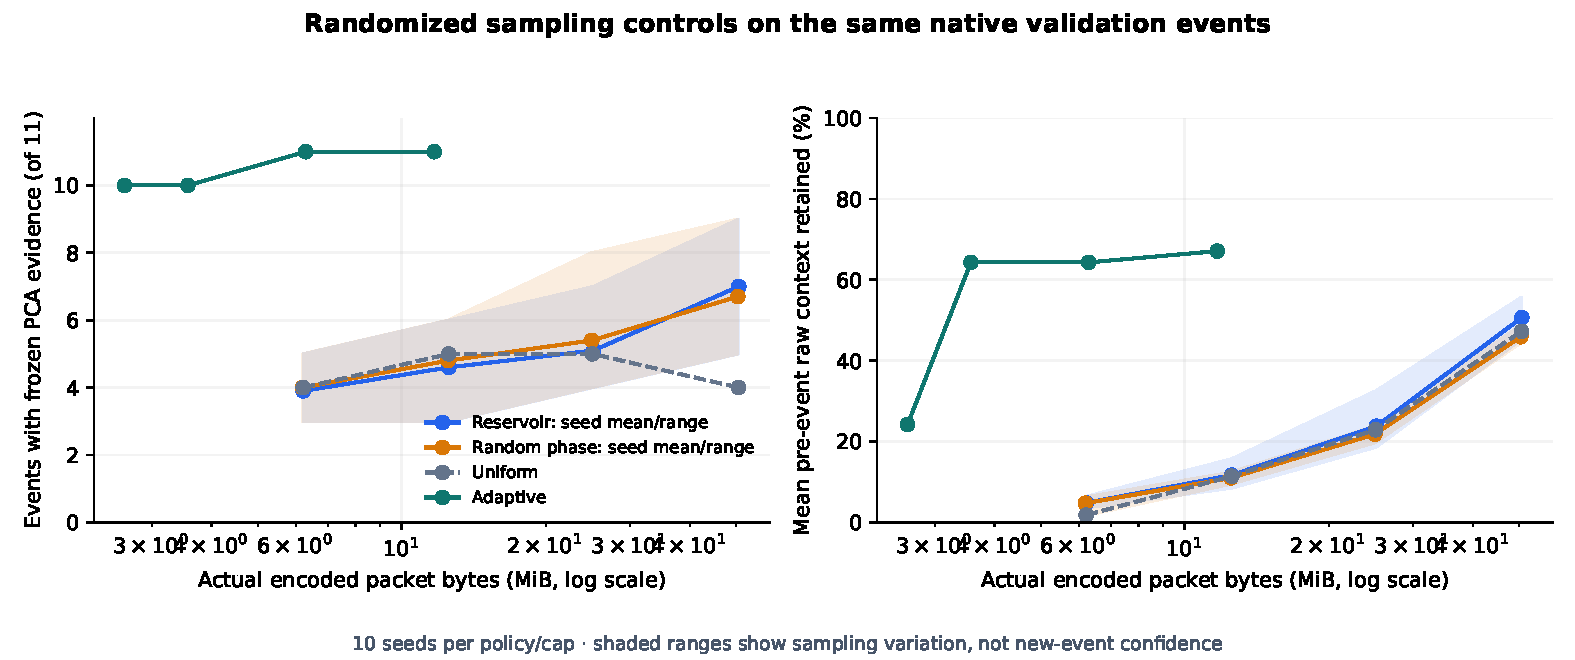
\includegraphics[width=\linewidth]{generated/randomized_tradeoff.pdf}
\caption{Mission1 evidence and context against actual encoded bytes. Shading is
the observed seed range, not a confidence interval for new faults. Shared caps
allow different actual expenditure.}
\label{fig:seeded}
\end{figure}

Sixteen paired ablation arms remove one component at a time. Full arms reproduce
the original adaptive packet bytes exactly. At 1,024 bytes, removing pre-trigger
capture preserves 11/11 PCA events while reducing pre-context from 64.3\% to 1.8\%.
Removing background reservation loses PCA evidence for event \texttt{id\_138} and
reduces cost from 6.30 to 0.90 MiB. At 256 bytes, releasing the background quota
instead increases pre-context from 24.2\% to 41.5\%. Thus reservation has a
budget-dependent opportunity cost. Removing post-trigger capture leaves PCA event
counts and pre-context unchanged at every cap; diagnostic post-event usefulness
has not been established. These removals do not estimate component interactions.

\subsection{Receiver mismatch and the temporal limitation}
\label{sec:mismatch}
The expanded benchmark crosses four capture conditions with threshold, adaptive,
and coverage recording, alongside uniform and seeded controls: 132 arms total.
At 1,024 bytes, adaptive and coverage retain rank-three PCA evidence for 11/11
events at approximately 6.30 MiB. Coverage raises pre-context from 64.3\% to
66.3\% but reduces post-context from 40.2\% to 36.9\%. At PCA ranks four and
five, coverage retains 11/11 and ordinary adaptive capture 10/11. With the trigger
disabled, their rank-three counts are 6/11 and 4/11 at 6.22 MiB. These are
correlated receiver sensitivities, not broad detector-independent guarantees.

The AR(1) receiver is calibrated on 8,712,785 eligible training pairs. Full-archive
input supplies evidence for all 11 events. Seven declared policies at four caps
give 28 temporal assessments. At 1,024 bytes, adaptive context preserves temporal
evidence for 10/11 events, uniform for 2/11, and threshold-only for 1/11. Disabled-
trigger singleton background retains 0/11 temporal events despite 4/11 PCA events.
Isolated retained values therefore cannot be treated as usable forecast transitions.

The pair control is introduced after observing that validation failure and assessed
in eight exploratory arms. Under enabled first-difference capture, it matches
adaptive's 10/11 temporal events at the 1,024-byte cap. With the trigger disabled,
it retains 2/11 temporal and 4/11 PCA events at 6.22 MiB. It partially addresses
the measured input failure without establishing optimal allocation or general
protection of unfamiliar faults. Table~\ref{tab:temporal} reports cost and input
availability alongside event counts; Figure~\ref{fig:requirements} contrasts this
development result with the frozen follow-up.

\begin{table}[htbp]
\centering\small
% Generated temporal receiver and adjacent-pair comparison.
\begin{tabular}{lrrrr}
\toprule
Capture / policy & MiB & PCA events & AR(1) events & Retained pairs \\
\midrule
Uniform & 25.04 & 5/11 & 2/11 & 2957 \\
Diff. / threshold & 0.81 & 10/11 & 1/11 & 11 \\
Diff. / adaptive & 6.30 & 11/11 & 10/11 & 1057 \\
Diff. / coverage & 6.30 & 11/11 & 10/11 & 4886 \\
Level / adaptive & 6.67 & 11/11 & 10/11 & 7281 \\
Pca / adaptive & 8.86 & 11/11 & 10/11 & 69167 \\
Disabled / adaptive & 6.22 & 4/11 & 0/11 & 0 \\
Diff. / burst & 6.30 & 11/11 & 10/11 & 79668 \\
Disabled / burst & 6.22 & 4/11 & 2/11 & 78877 \\
\bottomrule
\end{tabular}

\caption{Mission1 at 1,024 bytes per hour. Pairs require consecutive original
observations within the gap limit; input counts include periods excluded from
fault scoring. Burst rows are exploratory. Exact bytes and complete cap results
are in the reports.}
\label{tab:temporal}
\end{table}

\section{Seeded Sampling Controls}
\subsection{Policies and protocol}
To examine whether the initial comparison depended on deterministic sampling
alignment, we add reservoir sampling and randomized-phase uniform sampling.
The receivers, thresholds, original observations, eligibility rules, context
window, reporting epochs, and four byte caps remain unchanged. Receiver parameters
are loaded exactly from the completed pilot, not fitted again. Before reusing the
original controls, the runner verifies source/cache identity, receiver-file equality,
evaluation-source hashes, and every original packet stream's hash.

Reservoir sampling uses Algorithm R as reviewed by
\citet{vitter1985reservoir}. With raw capacity $K$, observation $i$ is stored while
$i\leq K$; subsequently a uniform integer $j\in\{0,\ldots,i-1\}$ replaces slot
$j$ when $j<K$. An unused draw is also made during the initial fill to couple
random draws across capacities without changing the marginal sampling rule.
Under ideal uniform draws, the final reservoir is a uniform sample without
replacement of $\min(K,N)$ observations. It uses bounded epoch state and does not
require the final observation count. Replacement before packet finalization is
causal because all policies deliver their packet at epoch end.

Randomized-phase uniform sampling draws an integer phase $\phi$ uniformly from
$\{0,\ldots,T-1\}$ and schedules target $j$ at offset $(jT+\phi)/K$. It retains
the first available observation at or after a target. A gap can skip several
targets but cannot cause a duplicate record; a target without a later observation
inside its epoch remains unfilled. Integer comparisons avoid timestamp-rounding
ambiguity. This is uniform sampling in time with randomized phase, not a claim
of equal inclusion probabilities for irregularly spaced observations.

Seeds 0--9 were enumerated before this comparison and all are reported. A generator
for each policy/seed/epoch is initialized from SHA-256 of those identifiers.
Budget is omitted to couple random numbers across caps. Skipping an earlier epoch
cannot shift another epoch's sequence. Budgets are correlated comparisons, and
reservoir sets across capacities need not be nested. The two policies, four caps,
and ten seeds produce 80 new arms. Capture workers receive observations and
randomization/configuration only; all capture finishes before annotation-based
decoded evaluation begins.

\subsection{Results and sampling variability}
\begin{table}[ht]
\centering\footnotesize
% Generated randomized validation comparison; seed ranges are not event confidence intervals.
\begin{tabular}{rlrrr}
\toprule
Cap & Policy & Mean MiB & PCA events: mean [range] & Context (\%) \\
\midrule
256 & Reservoir & 6.22 & 3.9 [3, 5] & 4.8 \\
256 & Random phase & 6.20 & 4.0 [3, 5] & 4.7 \\
512 & Reservoir & 12.54 & 4.6 [3, 6] & 11.7 \\
512 & Random phase & 12.49 & 4.8 [3, 6] & 11.0 \\
1024 & Reservoir & 25.15 & 5.1 [4, 7] & 23.8 \\
1024 & Random phase & 24.96 & 5.4 [4, 8] & 21.8 \\
2048 & Reservoir & 50.67 & 7.0 [5, 9] & 50.6 \\
2048 & Random phase & 50.44 & 6.7 [5, 9] & 45.9 \\
\bottomrule
\end{tabular}

\caption{Seeded validation comparisons. Actual expenditure and context are averaged
across all ten seeds. PCA counts are means and observed seed minima/maxima out of
the same 11 source-eligible events. These ranges are not confidence intervals for
new-event performance.}
\end{table}

At the 1,024-byte hourly cap, reservoir sampling retains frozen PCA evidence for
a mean of 5.1 events, with a seed range of 4--7, using 25.15 MiB on average.
Randomized phase retains a mean of 5.4, range 4--8, using 24.96 MiB. The original
adaptive arm retains 11 events using 6.30 MiB. Mean pre-event context coverage is
23.8\% for reservoir and 21.8\% for randomized phase, compared with 64.3\% for
adaptive capture. Thus the initial adaptive result remains favorable against these
two controls within the existing validation setting.

\begin{figure}[ht]
\centering
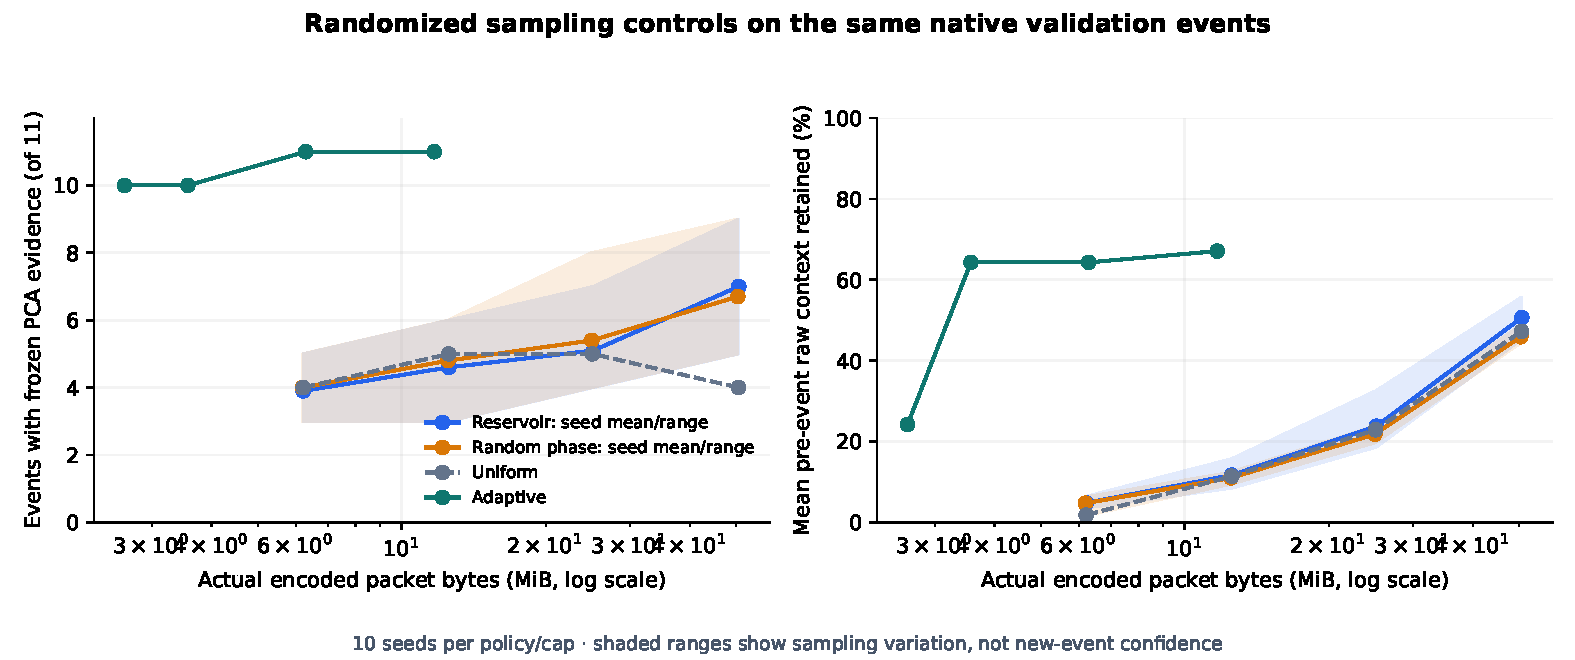
\includegraphics[width=\linewidth]{generated/randomized_tradeoff.pdf}
\caption{Means and observed seed ranges for randomized policies; original uniform
and adaptive curves are fixed controls. All methods share per-epoch byte caps,
not identical actual expenditure. Repeated seeds describe sampling variation on
this archive rather than additional independent spacecraft faults.}
\end{figure}

For the 1,024-byte streams, reservoir produces 8,016--8,125 positive normal PCA
observations and randomized phase 6,728--6,890, compared with 1,848 in the adaptive
arm. Different numbers of observations are scored, so these counts cannot be
interpreted as calibrated or comparable operational false-alarm episode rates.
The threshold-only control remains relevant: it spends 0.81 MiB and retains ten
events, exposing a cost/evidence tradeoff rather than a universal winner.

\subsection{Limits of the stronger comparison}
The ten seeds do not turn 11 events into 110 independent faults. We report every
seed and event-specific retention frequency without presenting the observed ranges
as generalization confidence intervals. The adaptive arm, including its background
sampling phase, is still deterministic. Its components have not been isolated by
this experiment. Stronger adaptive acquisition methods, component ablations,
receiver swaps, and a frozen independent-mission study remain necessary before
claims of novelty, robust diagnostic benefit, or broad superiority are warranted.

\section{Component Ablations and a Frozen Transfer Protocol}
\label{sec:ablations}
We replay the same native validation observations through the full adaptive
recorder and three single-component removals at each of the four caps (16 arms).
The receiver parameters, trigger threshold, context settings other than the removed
component, and event denominators remain fixed. Every full-arm packet stream is
byte-for-byte identical to its original pilot counterpart. Removing background
reservation releases its quota to trigger capture; this is a practical configuration
ablation under a shared cap, not an equal-expenditure or factorial interaction study.

\begin{table}[htbp]
\centering
\small
% Generated paired development ablations; caps are not equal expenditures.
\begin{tabular}{rlrrr}
\toprule
Cap & Variant & MiB & PCA events & Pre-context (\%) \\
\midrule
256 & Full & 2.63 & 10/11 & 24.2 \\
256 & No pre & 2.63 & 10/11 & 0.0 \\
256 & No post & 2.63 & 10/11 & 24.2 \\
256 & No background & 0.84 & 10/11 & 41.5 \\
512 & Full & 3.57 & 10/11 & 64.3 \\
512 & No pre & 3.55 & 10/11 & 1.8 \\
512 & No post & 3.56 & 10/11 & 64.3 \\
512 & No background & 0.88 & 10/11 & 64.3 \\
1024 & Full & 6.30 & 11/11 & 64.3 \\
1024 & No pre & 6.26 & 11/11 & 1.8 \\
1024 & No post & 6.28 & 11/11 & 64.3 \\
1024 & No background & 0.90 & 10/11 & 64.3 \\
2048 & Full & 11.69 & 11/11 & 67.1 \\
2048 & No pre & 11.66 & 11/11 & 9.1 \\
2048 & No post & 11.68 & 11/11 & 67.1 \\
2048 & No background & 0.90 & 10/11 & 64.3 \\
\bottomrule
\end{tabular}

\caption{Paired development ablations. Pre-context is the macro fraction of original
observations retained in each eligible event's five-minute pre-onset window.
All variants share 11 eligible events; actual expenditure differs.}
\label{tab:ablations}
\end{table}

At the 1,024-byte cap, removing pre-trigger capture preserves PCA evidence for
11/11 events while reducing pre-context coverage from 64.3\% to 1.8\%.
Thus event detection alone conceals a substantial loss of investigation context.
Removing background sampling reduces PCA evidence to 10/11 events and actual
expenditure from 6.30 to 0.90 MiB. Event \texttt{id\_138}, whose annotated span is
53,580 seconds, loses PCA evidence without background sampling. The same event is
lost at the 2,048-byte cap. At 256 bytes, removing background reservation instead
increases pre-context coverage from 24.2\% to 41.5\%, consistent with releasing
capacity for trigger context; the design has budget-dependent tradeoffs.

Removing post-trigger capture leaves PCA event counts and aggregate pre-context
coverage unchanged at all four caps, with small byte savings. This result does not
establish diagnostic value for post-trigger capture, nor its dispensability:
post-event reconstruction and operator diagnosis are not measured. These single
removals do not estimate interactions or establish a globally optimal allocation.
All results remain conditional on the same small development archive.

\paragraph{Independent mission protocol.}
A mission-neutral numerical bundle and a two-stage freeze/run interface now support
an independent evaluation. Before replay, the lock binds input-manifest and code
hashes to the fixed Mission1 retention settings, four caps, and ten seeds. The
new mission's receiver normalization, PCA basis, and score thresholds are calibrated
only on its designated training observations. This evaluates transfer of retention
settings with training-calibrated receivers, not zero-shot receiver transfer.
Training and evaluation annotations are stored separately; evaluation annotations
are parsed only after all packet streams have been captured. The original retention-only interface reports 108 policy,
ablation, and seed arms, together with a full-archive reference. The extended
receiver-mismatch interface is described in Section~\ref{sec:mismatch}.
Descriptive event strata are fixed at durations of at most 60 seconds, over 60
through 600 seconds, and over 600 seconds, and adjacent eligible-observation gaps at a 150-second
boundary (annotation exclusions can contribute to these gaps). Small strata are not independent estimates of generalization uncertainty.

The interface currently requires six synchronized native channels and retains the
existing byte schema. Asynchronous observations and arbitrary channel counts remain
unsupported. Channel selection and split decisions must be documented before
examining evaluation outcomes. Hash locks expose accidental changes but cannot
prove prior label blindness or replace a public experimental record. The interface has been exercised on synthetic fixtures only; an independent-mission result remains pending.

\section{Capture Mismatch, Temporal Evidence, and Delivery}
\label{sec:mismatch}
The mismatch experiment asks whether retained observations remain useful
when the downstream receiver differs from the capture trigger. We compare
first-difference, standardized-level, and PCA-guided capture, plus an explicitly
disabled trigger as a stress control. Level capture uses the existing six-standard-
deviation threshold; PCA capture reaches the same trigger boundary at its frozen
training score quantile. Each condition drives threshold-only capture, the existing
adaptive recorder, and a coverage-based background control. Uniform and ten-seed
reservoir/random-phase controls complete 132 arms across the four caps.
Original pilot and seeded streams are hash-verified and reused.

The receiver bank contains standardized level and PCA residuals at ranks one
through five. All additional calibration uses eligible training observations only;
the original level and rank-three parameters remain exact. PCA ranks are correlated
sensitivity checks, not independent detector families or fault examples. All
source-eligible events stay in the denominator, and each receiver separately reports
full-archive recoverability and losses caused by retention.

\paragraph{Coverage control.}
Within each reserved background time stratum, a bounded candidate replaces its
background observation when a new observation is further from the already retained
background observations in frozen standardized units. Records requested by trigger
or context capture are protected. The candidate uses the same reserved quota and
wire schema. This is an experimental diversity control, not a claim of a novel
streaming selection algorithm or an optimal allocation.

\begin{table}[htbp]
\centering
\scriptsize
% Generated from completed receiver mismatch benchmark.
\begin{tabular}{llrrrr}
\toprule
Capture & Policy & MiB & PCA events & Blind kept/available & Pre-context (\%) \\
\midrule
Difference & Threshold & 0.81 & 10/11 & 0/1 & 0.0 \\
Difference & Adaptive & 6.30 & 11/11 & 1/1 & 64.3 \\
Difference & Coverage & 6.30 & 11/11 & 1/1 & 66.3 \\
Level & Threshold & 1.38 & 10/11 & 0/1 & 0.0 \\
Level & Adaptive & 6.67 & 11/11 & 1/1 & 65.1 \\
Level & Coverage & 6.67 & 11/11 & 1/1 & 67.1 \\
PCA & Threshold & 1.58 & 11/11 & 0/0 & 0.0 \\
PCA & Adaptive & 8.86 & 11/11 & 0/0 & 65.1 \\
PCA & Coverage & 8.75 & 11/11 & 0/0 & 66.3 \\
Disabled & Threshold & 0.80 & 0/11 & 0/11 & 0.0 \\
Disabled & Adaptive & 6.22 & 4/11 & 4/11 & 1.8 \\
Disabled & Coverage & 6.22 & 6/11 & 6/11 & 2.9 \\
\bottomrule
\end{tabular}

\caption{Capture mismatch at the 1,024-byte hourly cap. ``Blind'' means no
capture threshold crossing within the event; nearby triggers can still preserve
context. The conditional denominator includes only full-archive PCA-recoverable
events. All 11 source-eligible events remain in the overall event denominator.}
\label{tab:mismatch}
\end{table}

With first-difference capture, both adaptive and coverage recorders retain
rank-three PCA evidence for 11/11 events at approximately 6.30 MiB. Coverage
increases pre-context from 64.3\% to 66.3\% but reduces post-context from 40.2\%
to 36.9\%. At ranks four and five, the original adaptive recorder retains 10/11
events and the coverage control retains 11/11. With the trigger disabled, they
retain rank-three evidence for 4/11 and 6/11 events respectively at 6.22 MiB.
These differences concern the same small validation archive, not evidence of
robustness to an arbitrary future model.

\paragraph{A distinct temporal receiver.}
We fit a ridge AR(1) model on 8,712,785 eligible consecutive training pairs,
with regularization 0.001, a 150-second gap reset, and a training score quantile
of 0.999. Scores use standardized forecast residuals. Both original endpoints
must survive for a transition to supply evidence: retained samples separated by
discarded observations are never silently stitched together. The full archive
contains temporal evidence for all 11 eligible events. Seven declared policies
at four caps give 28 temporal evaluations.

At 1,024 bytes, the existing adaptive recorder retains temporal evidence for
10/11 events, compared with 2/11 for uniform and 1/11 for threshold-only capture.
Disabling the trigger leaves singleton adaptive background capture with 0/11
temporal events despite its 4/11 pointwise PCA result. This exposes a limitation
of equating isolated retained values with evidence for a temporal receiver.

After observing this validation failure, we implement an adjacent-pair background
control and run eight exploratory arms. It reserves the same fraction of raw
capacity for pairs within time strata, rejects partners beyond the gap limit,
and never pairs across epochs. Odd unused quota slots remain unfilled. With
first-difference triggers, it retains 10/11 temporal events at the 1,024-byte cap,
matching the original recorder. With the trigger disabled, it retains 2/11 temporal
and 4/11 PCA events at 6.22 MiB. This partially addresses the measured failure,
not the general problem of preserving every unfamiliar fault. Its design is
informed by validation outcomes and requires independent confirmation.

\begin{table}[htbp]
\centering
\small
% Generated temporal receiver and adjacent-pair comparison.
\begin{tabular}{lrrrr}
\toprule
Capture / policy & MiB & PCA events & AR(1) events & Retained pairs \\
\midrule
Uniform & 25.04 & 5/11 & 2/11 & 2957 \\
Diff. / threshold & 0.81 & 10/11 & 1/11 & 11 \\
Diff. / adaptive & 6.30 & 11/11 & 10/11 & 1057 \\
Diff. / coverage & 6.30 & 11/11 & 10/11 & 4886 \\
Level / adaptive & 6.67 & 11/11 & 10/11 & 7281 \\
Pca / adaptive & 8.86 & 11/11 & 10/11 & 69167 \\
Disabled / adaptive & 6.22 & 4/11 & 0/11 & 0 \\
Diff. / burst & 6.30 & 11/11 & 10/11 & 79668 \\
Disabled / burst & 6.22 & 4/11 & 2/11 & 78877 \\
\bottomrule
\end{tabular}

\caption{Temporal receiver comparison at 1,024 bytes per hour. Retained pairs
require consecutive original observations within the gap limit. Burst rows are
exploratory additions after inspecting the temporal validation result.}
\label{tab:temporal}
\end{table}

\paragraph{Delivered rather than merely captured evidence.}
A store-and-forward simulator adds finite payload buffers, drop-oldest/drop-newest
rules, discrete contacts, partial transfer progress, framing costs, and completed-
packet loss. Arrivals at epoch end enter before service at the same timestamp.
Undelivered packets at evaluation end provide no evidence. Packet and payload
conservation are checked, and only completely delivered packets reach evaluation.
The model abstracts physical frame timing and does not implement retransmission.

Illustrative contacts occur every six hours. Ample/lossy conditions allow 32,768
wire bytes per contact and a 16,384-byte payload buffer; congestion allows 2,048
and 4,096 bytes. Every 128 payload bytes incur 16 framing bytes. The lossy case
uses probability 0.1 and one declared seed. At 1,024 bytes, congestion reduces
uniform PCA evidence from 5/11 to 4/11 while adaptive and coverage retain 11/11;
the lossy realization reduces both latter policies to 10/11. These schedules
are not validated mission requirements and one loss seed is not an uncertainty
analysis. Congestion differences combine selection with differing actual
expenditure; they do not isolate transport robustness at matched byte cost. Buffer limits exclude Python object metadata.

\begin{table}[htbp]
\centering
\small
% Generated finite-buffer delivery comparison.
\begin{tabular}{llrrr}
\toprule
Policy & Link & Wire MiB & Delivered packets & PCA events \\
\midrule
Uniform & Ample & 28.24 & 26304/26304 & 5/11 \\
Uniform & Congested & 8.56 & 4498/26304 & 4/11 \\
Uniform & Lossy & 28.24 & 23638/26304 & 5/11 \\
Adaptive & Ample & 7.11 & 26304/26304 & 11/11 \\
Adaptive & Congested & 7.04 & 26182/26304 & 11/11 \\
Adaptive & Lossy & 7.11 & 23638/26304 & 10/11 \\
Coverage & Ample & 7.11 & 26304/26304 & 11/11 \\
Coverage & Congested & 7.04 & 26182/26304 & 11/11 \\
Coverage & Lossy & 7.11 & 23638/26304 & 10/11 \\
\bottomrule
\end{tabular}

\caption{Encoded evidence after illustrative finite-buffer delivery, at the
1,024-byte hourly recording cap. Wire cost includes framing and unsuccessful
or partial transmissions; it differs from encoded capture expenditure.}
\label{tab:delivery}
\end{table}

\begin{figure}[htbp]
\centering
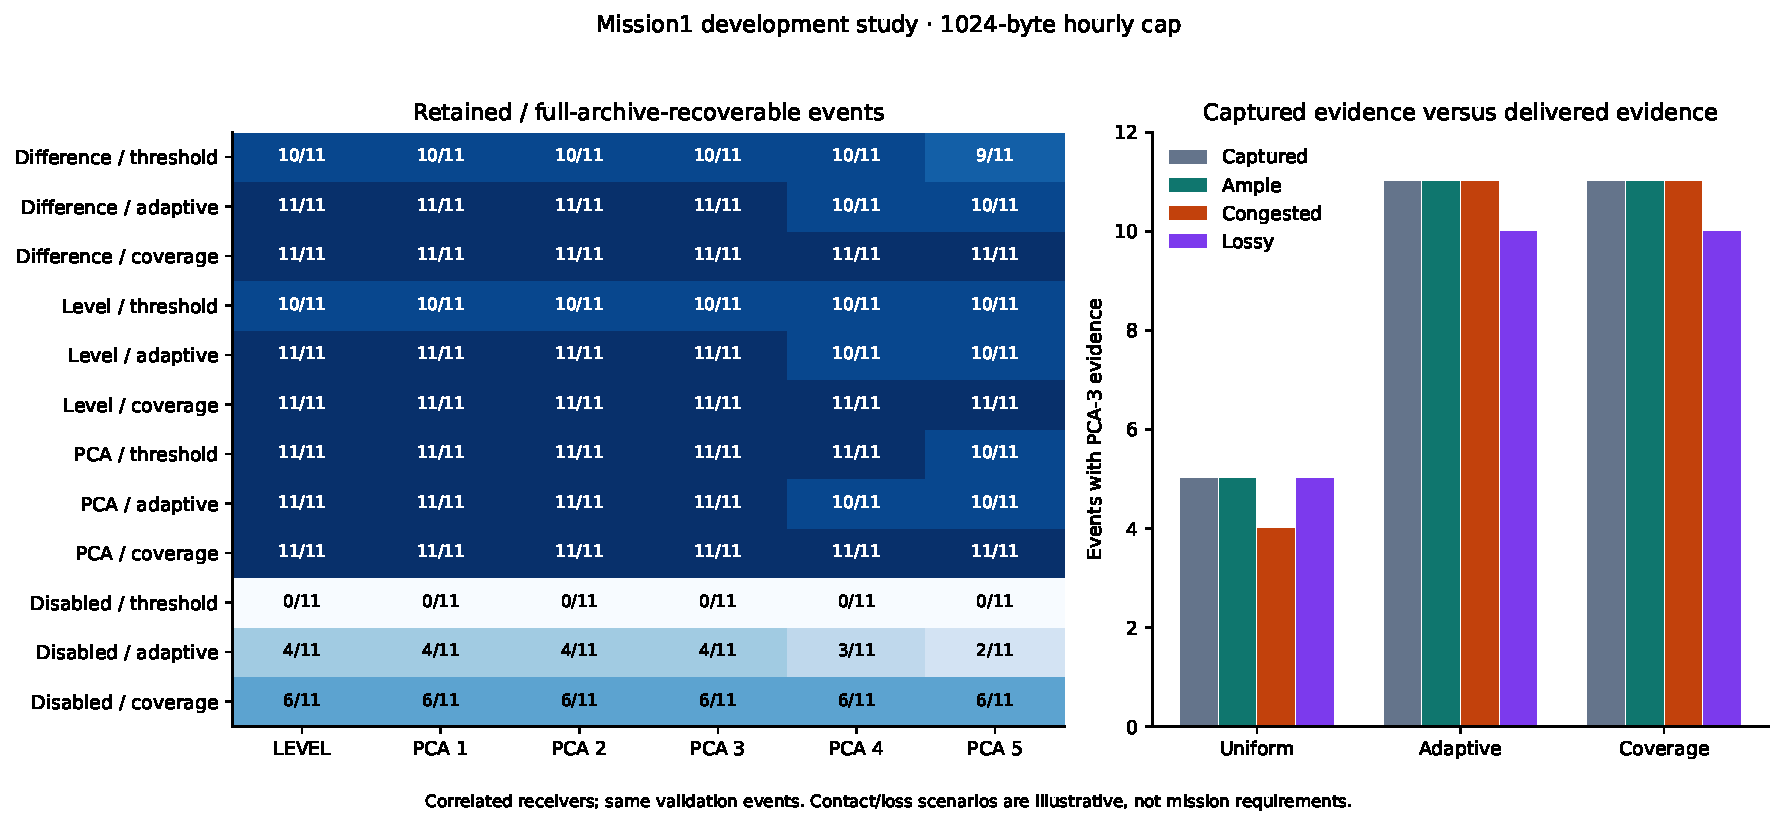
\includegraphics[width=\linewidth]{generated/receiver_mismatch.pdf}
\caption{Receiver sensitivity and captured/delivered evidence on the same
Mission1 validation events. Matrix denominators are receiver-specific full-archive
recoverability. Neither the correlated receivers nor the link scenarios establish
independent-mission generalization.}
\label{fig:mismatch}
\end{figure}

\paragraph{Reproducibility and resource scope.}
The independent-mission benchmark now locks input, canonical settings, code and
requirements hashes, and Python/NumPy versions. It reports 148 default capture
arms including adjacent-pair controls, followed by 36 selected temporal evaluations.
Only synthetic external bundles have been exercised; an independent mission result
remains pending. A separate 20,000-observation host profile measures replay timing
and Python-traced allocations in different passes. On this local run, adaptive
replay processes approximately 396,000 observations per second and coverage
approximately 104,000, including synthetic sample construction, encoding, and
hashing. These are single-run host measurements under a local development
workload, not embedded latency, total RAM, or flight suitability evidence.

\section{Limitations and Work Required before Submission}
The native pilot provides validation retention measurements, but no independent
mission generalization or operator diagnostic benefit has yet been established.
The synthetic events are few, simple, and known to the experiment designer. A
summary's coarse overlap can associate unrelated extrema with an event, while
raw event coverage says little about physical diagnosis. Neither is sufficient
as the sole scientific endpoint.

A recorder guided by anomaly scores inherits model blind spots. Reserved
background sampling mitigates this structurally but offers no guarantee of
capturing every unfamiliar event. The current reservation is deterministic,
context is counted in samples rather than elapsed time, and rings reset at epoch
boundaries. Budget exhaustion is first-come rather than an optimized eviction
policy. Seeded controls examine alignment sensitivity, and single-component ablations
examine the current adaptive choices. Component interactions, operator utility,
and stronger established adaptive competitors remain untested.

The packet format excludes physical link overhead. A separate simulator charges
illustrative framing and finite-buffer contacts, but its schedule is not grounded
in a mission requirement and its single loss seed does not support uncertainty claims.
Driver memory use is not onboard memory use, and Python execution says little
about flight suitability. Asynchronous channels, stronger temporal receivers, hardware measurements, and
validated contact requirements remain future work. The AR(1) receiver is a simple
linear baseline, and the adjacent-pair control was designed after inspecting the
same validation archive. The retention experiments run entirely in Python. A native recorder is justified only if
profiling or an embedded deployment claim requires it.

A publishable revision requires an expanded prior-art review, an independent
mission evaluation with frozen decisions, official ESA scoring where applicable,
a matched resource-budget study, and operational requirements from a collaborating
engineering team. Affiliation, venue, data permissions, and any funding, conflict, or required
AI-assistance disclosures must be confirmed before circulation as a submission.

\section{Conclusion}
Telemetry retention should be evaluated by the evidence available after decoding
and delivery, including the inputs required by the downstream receiver. In this
Mission1 development study, adaptive capture preserves more frozen-receiver event
evidence and pre-event context than the tested uniform and seeded sampling
controls under common byte caps. Component removals show that an unchanged event
count can conceal substantial context loss. Receiver mismatch reveals a second
limitation: isolated background observations can preserve pointwise evidence while
providing no usable transitions to a forecasting receiver. An adjacent-pair control
partially addresses that failure in an exploratory validation experiment.

The practical result is an auditable evaluation framework and a specific research
question: which retention choices preserve useful evidence when the downstream
model changes? The present results do not settle that question across missions or
establish a novel optimal recorder. Independent evaluation, stronger established
comparisons, and operator assessment are the next sources of evidence.
\section*{Reproducibility and Data Availability}
Code, compact JSON reports, full arm/per-event records, protocol text and locks,
generated figures/tables, and this report are maintained in the project
repository:\footnote{\url{https://github.com/simonbalanoff/telemetry-anomaly-engine}.}
The data source is the official ESA release~\citep{esa2025dataset}; original archives
and large arrays/packet streams are obtained or generated separately and are not
redistributed. Source hashes bind each native export and bundle to its inputs.
The Mission2 report records the lock commit and verifies it again before temporal
assessment and primary analysis. The local Git record makes changes traceable but
cannot prove prior label blindness or substitute for public preregistration.

The implementation uses Python, NumPy, and pandas; plotting uses Matplotlib. The
benchmark guide documents source preparation, capture, calibration, decoded
assessment, and transport assumptions. Small synthetic integration cases run
without mission data. The current 111-test suite includes budget and chronology
invariants, native-value checks, split-edge censorship, input/code tampering,
committed-protocol barriers, and empty-denominator handling. Software tests do
not establish scientific generalization. Experiment reports record their numerical
environment and refuse to overwrite completed outputs.

All numerical tables are generated from completed reports. The Mission2 primary
analysis is preserved separately from post-evaluation annotation-support and
presentation checks. The latter independently verifies that raw CSV categories and
split intersections agree with the prepared bundle; it does not select another
subset or alter scoring. A snapshot manifest binds the repository PDF and preview
to the manuscript, bibliography, generated tables, and figures. Version 1.0
contained Mission1 evidence only; this revision adds the complete Mission2 attempt
and narrows the generalization claim accordingly.


\paragraph{Preparation assistance.}
AI-assisted tools supported software implementation and manuscript drafting.
This technical report has not undergone peer review or operational validation.

\bibliographystyle{plainnat}
\bibliography{references}
\clearpage
\appendix
\section{Synthetic Validation and Software Invariants}
\label{app:checks}
The synthetic scenario validates serialization and causal recorder behavior.
It is a software check, separate from the native mission comparisons.


The reproducible smoke scenario has 360 six-channel observations at five-second
intervals over three ten-minute epochs. Seed 2026 fixes Gaussian background noise.
A point spike, a sustained step, and a slow ramp are injected at declared times.
Each epoch has a 1,024-byte cap. Capture uses a first-difference threshold of 2;
the receiver uses an amplitude threshold of 4. The adaptive ring and post-trigger
window each contain three samples, with $\rho=0.2$ background reservation.
These settings are illustrative and were not selected on mission data.

\begin{table}[ht]
\centering
\footnotesize
% Generated by python/run_retention_demo.py; synthetic checks only.
\begin{tabular}{lrrrr}
\toprule
Policy & Bytes & Raw records & Raw event coverage & Receiver evidence \\
\midrule
Uniform & 3012 & 81 & 2/3 & 2/3 \\
Summaries & 2976 & 0 & 0/3 & 3/3 \\
Threshold & 276 & 5 & 2/3 & 2/3 \\
Adaptive & 1680 & 44 & 3/3 & 3/3 \\
\bottomrule
\end{tabular}

\caption{Synthetic protocol check only. Each policy has the same three-epoch
allocation of 3,072 bytes. Raw event coverage here counts events with at least
one retained raw observation, not a per-event sample fraction. Receiver evidence
for summaries is coarse bucket evidence. Actual expenditure differs by policy.}
\label{tab:smoke}
\end{table}

The artifact checks packet-byte limits, decoding, timestamp fidelity, bounded
record counts, background reservation under continuous triggering, and causal
prefix behavior. Tests also reject invalid input, malformed packets, duplicate
raw timestamps, and budget reset through reopening a finalized epoch.
Table~\ref{tab:smoke} is generated directly from the recorded experiment artifact.
It is not a statistical comparison, a diagnosis study, or a claim that the proposed
policy outperforms established mission recorders.

\end{document}
